\chapter{Knowledge-Based System Extraction from Deep Learning Models}
\label{chap:kbsextractiondl}
%ENLAZAR ESTO CON LOS PRINCIPIOS DE EXPLICABILIDAD DE PHILLIPS ET AL..
\blfootnote{Elvira Amador-Domínguez, Emilio Serrano, & Daniel Manrique (2021). A hierarchical multi-agent architecture based on virtual identities to explain black-box personalization policies. Expert Syst. Appl., 186, 115731. doi:10.1016/j.eswa.2021.115731}


\section{Knowledge Extraction from Deep Learning Models}\label{6_sec:kbs_extra_dl_method}
In this context, the DL model acts as a passive element, from which KBS is extracted by means of a middleware model. Method design parameters for KBS extraction from DL models are depicted in Figure \ref{fig:kbs_extra_dl_overview}.
\begin{figure}[t]
    \centering
    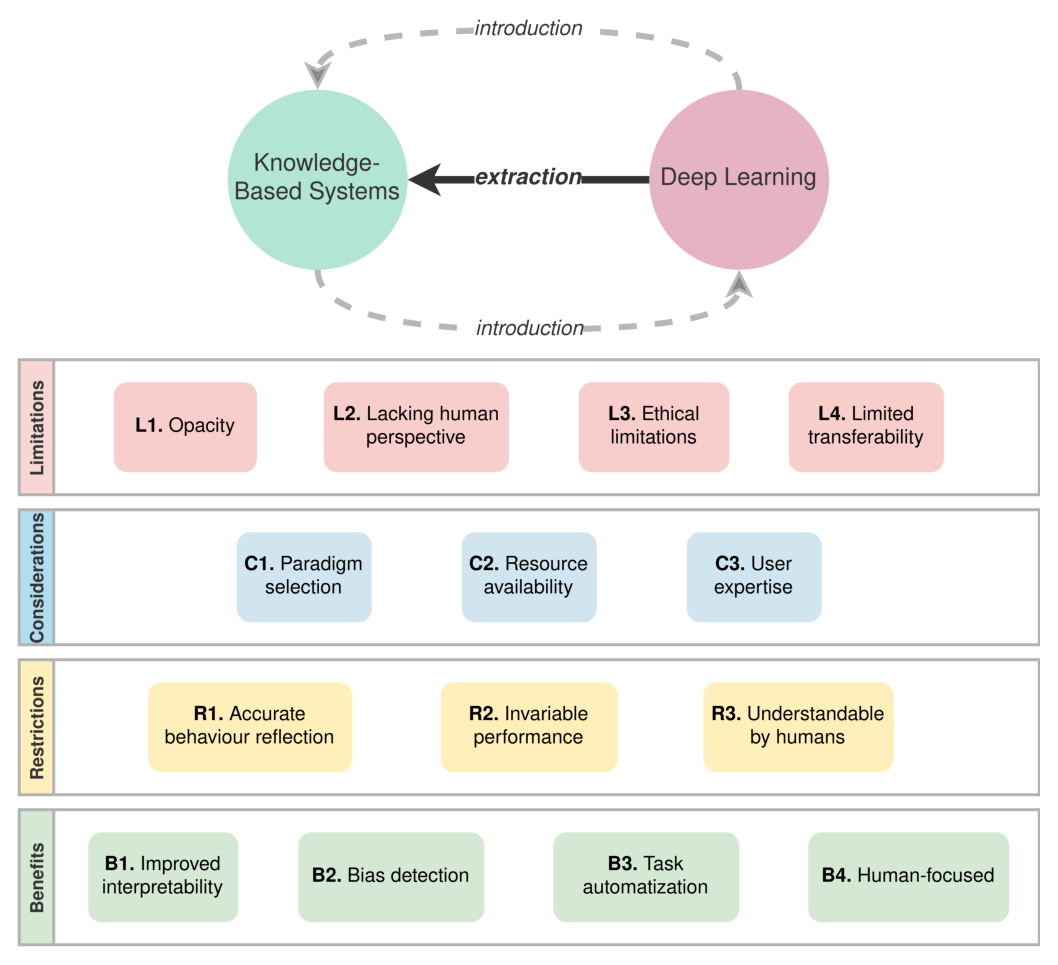
\includegraphics[width=\linewidth]{6_kbsextractiondl/figures/K_extraction_DL.eps}
    \caption{Overview on the Extraction of Knowledge-Based Systems from Deep Learning Models}
    \label{fig:kbs_extra_dl_overview}
\end{figure}

\paragraph{Limitations}
\begin{enumerate} [start=1,label={\bfseries L\arabic*.}]
    \item \textbf{Opacity.} \label{kbsextradl_L_opacity} As outlined in the limitations of KBS insertion in DL (Section \ref{4_sec:methodology_kbs_intro_dl}, \ref{kbsintrodl_L_opacity}), opacity is one of the main drawbacks of DL models. While some recent efforts aim to provide an insight on the inference process followed by a DL model to generate a certain output from a given input, these insights are only approximated. Therefore, explainations can reliably capture the behaviour of the DL model, but it cannot be fully ascertain that they are an accurate depiction of the DL model's internal behaviour.

    \item \textbf{Lacking human perspective.} \label{kbsextradl_L_human} DL models are devised to operate autonomously, without the need of human intervention. This phenomenon may be beneficial in some scenarios, but it may be detrimental in those scenarios where user perspective is important. Such is the case of health related scenarios, where only expert users make final decisions, as DL model predictions may not be fully trusted or justified. 
    
    \item \textbf{Ethical limitations.} \label{kbsextradl_L_ethical} DL models infer patterns entirely from training data. Therefore, the inferred patterns are not subject to any ethical considerations. This issue is particularly concerning, as biases within the data can lead to the inference of patterns that may be discriminating or exhibit some ethical concerns.
    
    \item \textbf{Limited transferability.}\label{kbsextradl_L_transferability} The lack of understanding on the internal behaviour of DL models not only conditions its interactions with users, but also between models. This hinders the transferability of DL models, as it can not be ascertain beforehand how a model will behave on a different scenario.
\end{enumerate}

\paragraph{Considerations}
\begin{enumerate} [start=1,label={\bfseries C\arabic*.}]
    \item \textbf{Paradigm selection.} \label{kbsextradl_C_paradigm} KBS extraction from DL usually requires from one or more middleware models that perform the extraction and the conversion. Therefore, these models must be aligned with both the final KBS and the initial DL model. Moreover, if the KBS is devised as an explanatory mean for the DL model, it is also key to select a type of KBS that can accurately depict its behaviour.
    
    \item \textbf{Resource availability.} \label{kbsextradl_C_resource} As evidenced in the previous interactions, the inclusion of DL models generally carries an additional computational cost. In this scenario, where the DL model is a passive element, its computational cost may not be as remarkable. However, the introduction of middleware models may increase the resource demand. Providing the involved models with sufficient computational resources is therefore essential.
    
    \item \textbf{User expertise.} \label{kbsextradl_C_user} In explainability, the user replaces the DL model as the central element. Therefore, the extracted KBS should not only be aligned with the DL model, but also should be aligned with the final user. User expertise is an essential element in this scenario, as it conditions the KBS selection and behaviour.
\end{enumerate}

\paragraph{Restrictions}
\begin{enumerate} [start=1,label={\bfseries R\arabic*.}]
    \item \textbf{Accurate behaviour reflection.} \label{kbsextradl_R_behaviour} If the KBS serves explainatory purposes, then it must be an accurate reflection of the behaviour of the DL model. This implies that the KBS should not be considered a replacement for the DL model, nor improve its performance. The KBS must therefore imitate the behaviour of the DL model, which entails that the predictions of both models (correct and incorrect) must be similar.
    
    \item \textbf{Invariable performance.} \label{kbsextradl_R_performance} As previously described, the DL model plays a passive role in this interaction.  Whether the DL model serves as a source for KBS extraction, or acts as a black-box element to be explained, its performance must remain invariant and unaffected. This is particularly important regarding explainability, as modifications in the DL model may compromise their integrity, leading to inaccurate insights on its behaviour. 
    
    \item \textbf{Human-understandable.} \label{kbsextradl_R_human} KBS are inherently symbolic, producing outputs that are human-readable. However, as denoted in \ref{kbsextradl_C_user}, the understability of the output does not only depend on the model, but on the expertise of the final user. Therefore, KBS must not only be readable, but understandable by humans.
\end{enumerate}

\paragraph{Benefits}
\begin{enumerate} [start=1,label={\bfseries B\arabic*.}]
    \item \textbf{Improved interpretability.}\label{kbsextradl_B_interpretability} Opacity is one of the main hardships regarding DL models (\ref{kbsextradl_L_opacity}). Gaining knowledge on the inference process of DL models increases the trust that users may have on the model (\ref{kbsextradl_L_human}). Moreover, it can serve as a scaffold for improving the transferability of the model (\ref{kbsextradl_L_transferability}).
    
    \item \textbf{Bias detection.}\label{kbsextradl_B_bias} Inference patterns learned by DL models are solely based on the input training data. Data is subject to errors, and biases, which may cause the model to learn inferential patterns that, while accurate from a computational standpoint, may not be ethically correct (\ref{kbsextradl_L_ethical}). Becoming aware on the basis on which inference is performed may enable the detection of biases within the data, which can then be corrected.
    
    \item \textbf{Task automatization.}\label{kbsextradl_B_automatization} In addition to the explainability perspective, KBS extraction from DL can also be treated as a means for automatizing several tasks. In Section \ref{sec:sota_knowledge_extraction_dl}, ontology learning was presented as one of these cases, where ontologies were automatically mined. This approach can be taken for the automatization of different tasks, reducing the human effort required to perform them (\ref{kbsextradl_L_human}).
    
    \item \textbf{Human-focused.}\label{kbsextradl_B_human} DL models work virtually autonomously, minimizing the implication of users within the process. Making the models understandable by humans can increase the active implications of users within the learning process not only increasing their trust, but also enhancing the performance of the model from the inclusion of human knowledge (\ref{kbsextradl_L_human}). 
\end{enumerate}
%%HAY DOS CASOS DE USO. DAME TU FUERZA PEGASO QUE SE VIENE LA MADRE DE TODOS LOS INVENTS. 
\section{User Profiling and Privacy Protection from Black-Box Hyperpersonalization Models}\label{6_sec:mas_bbhos_general}

One of the main assets of DL models is their capacity to efficiently process vast amounts of heterogeneous data. Online marketing is one of the prominent areas where DL models are predominant, as they can ingest data from several data sources and generate accurate, fast responses. With the improvement of DL, marketing personalization policies have evolved from simpler statistical approaches, such as collaborative filtering, to the denominated \textit{hyper-personalization policies}. While classic personalization techniques group users by general, static traits (e.g. age, location), hyper-personalization policies incorporate dynamic and unique data about users (e.g. navigation data, sensor information). Hyper-personalization policies may improve user experience, but can raise some concerns, especially from the privacy protection perspective:

\subsection*{Opacity}
User data is the scaffold in which hyper-personalization policies are built. Some data is actively provided by the users from their publications in social media. However, a considerable amount of data still comes from mobile sensors and online activity, which is retrieved passively and unbeknownst to the user. Subsequently, when the user is faced with recommendations based solely on passively retrieved data, it can create a sense of rejection founded in a privacy invasion.

\subsection*{Limited adaptability} 
Hyper-personalization systems should be capable of automatically adapting to the user's needs. These changes may be detected from abrupt shifts in the user's data, causing the system to modify its behaviour accordingly. However, there is generally a delay between the time when the user develops a new interest and when the system changes. Elevated delays may deter the user. Actively involving the user in the changing process may be a solution to this issue.

\subsection*{Lack of privacy}
Determining the optimal level of specificity for each user is a complex and challenging task. The accepted degree of personalization may vary between users. Thus, techniques for some users may be acceptable, may be perceived as invassive for others. It is therefore crucial to ensure that the user feels comfortable with the level of personalization.

\subsection*{Absence of user input}
Users are at the core of hyper-personalization systems, whose goal is to accurately predict their needs. However, even though users are the most relevant component of these systems, their actual influence is minimal. Taking a hybrid approach, where the user actively participates in the personalization process, may not only create a sense of comfortableness, but enhance the behaviour of the model.

A multi-agent system (MAS) based on virtual identities integrating user input is proposed to tackle the aforementioned issues. The MAS serves as an intermediary between the user and the \textit{black-box hyperpersonalization online systems} (BBHOS), thus hindering the recollection of passive data and improving user privacy. Additionally, the main goal of the proposed MAS is to analyze the behaviour of BBHOS, extracting patterns on the responses of the system when faced with different user profiles. \textit{Generated virtual identities} (GVIDs) emulate the behaviour of real-life users, each with a unique profile formed from a combination of predefined traits and dynamic information (e.g. contextual information, social media data). The MAS orchestrates the interactions between the GVIDs and the BBHOS, gathering a set of tailored responses for each GVID profile. Although BBHOS are opaque, general associative patterns between the profiles represented by each GVID and the responses generated for each of them can be inferred. These patterns can superficially explain the behaviour of the BBHOS.

The knowledge extracted from these user profiling patterns can then be used for two different purposes: enhancing the privacy of the user and improving the relevance of the provided content. In the proposed system, the real user is masked by an agent, referred to as \textit{user virtualized identity} (UVID). The UVID acts as a surrogate, interacting with the BBHOS while simultaneously preventing the system from extracting information about the real user. While GVIDs have a passive role, being autonomously triggered and not interacting directly with the user, the UVID has an active role. Subsequently, the UVID is the only virtual identity able to perform certain transactions with the BBHOS. The proposed MAS adopts a hybrid solution, combining user interaction with autonomous behaviour to achieve a balance between adaptability and user reliability. In addition to triggering certain transactions, the user input also determines the validity of the personalized content provided by the BBHOS.

\subsection{A Hierarchical Multi-Agent Architecture Based on Virtual Identities}\label{6_sec:subsec:mas_description}

The proposed four-layered MAS that implements the proposal is depicted in Figure \ref{fig:overview_mas}. Each layer comprises a set of agents that perform a series of actions specific to each layer. Agents can communicate with other agents both from the same and adjacent layers. In addition to the MAS layers, a storage layer is included to store and manage the collected data. Layers can be grouped into two levels: autonomous and user-triggered. The autonomous level of the system aggregates the first two layers, which comprises those actions that execute without any user interaction and prepare the system for its subsequent use. The user-triggered level, associated with layers three and four, is reliant on the user to execute. 

\begin{figure}[t]
    \centering
    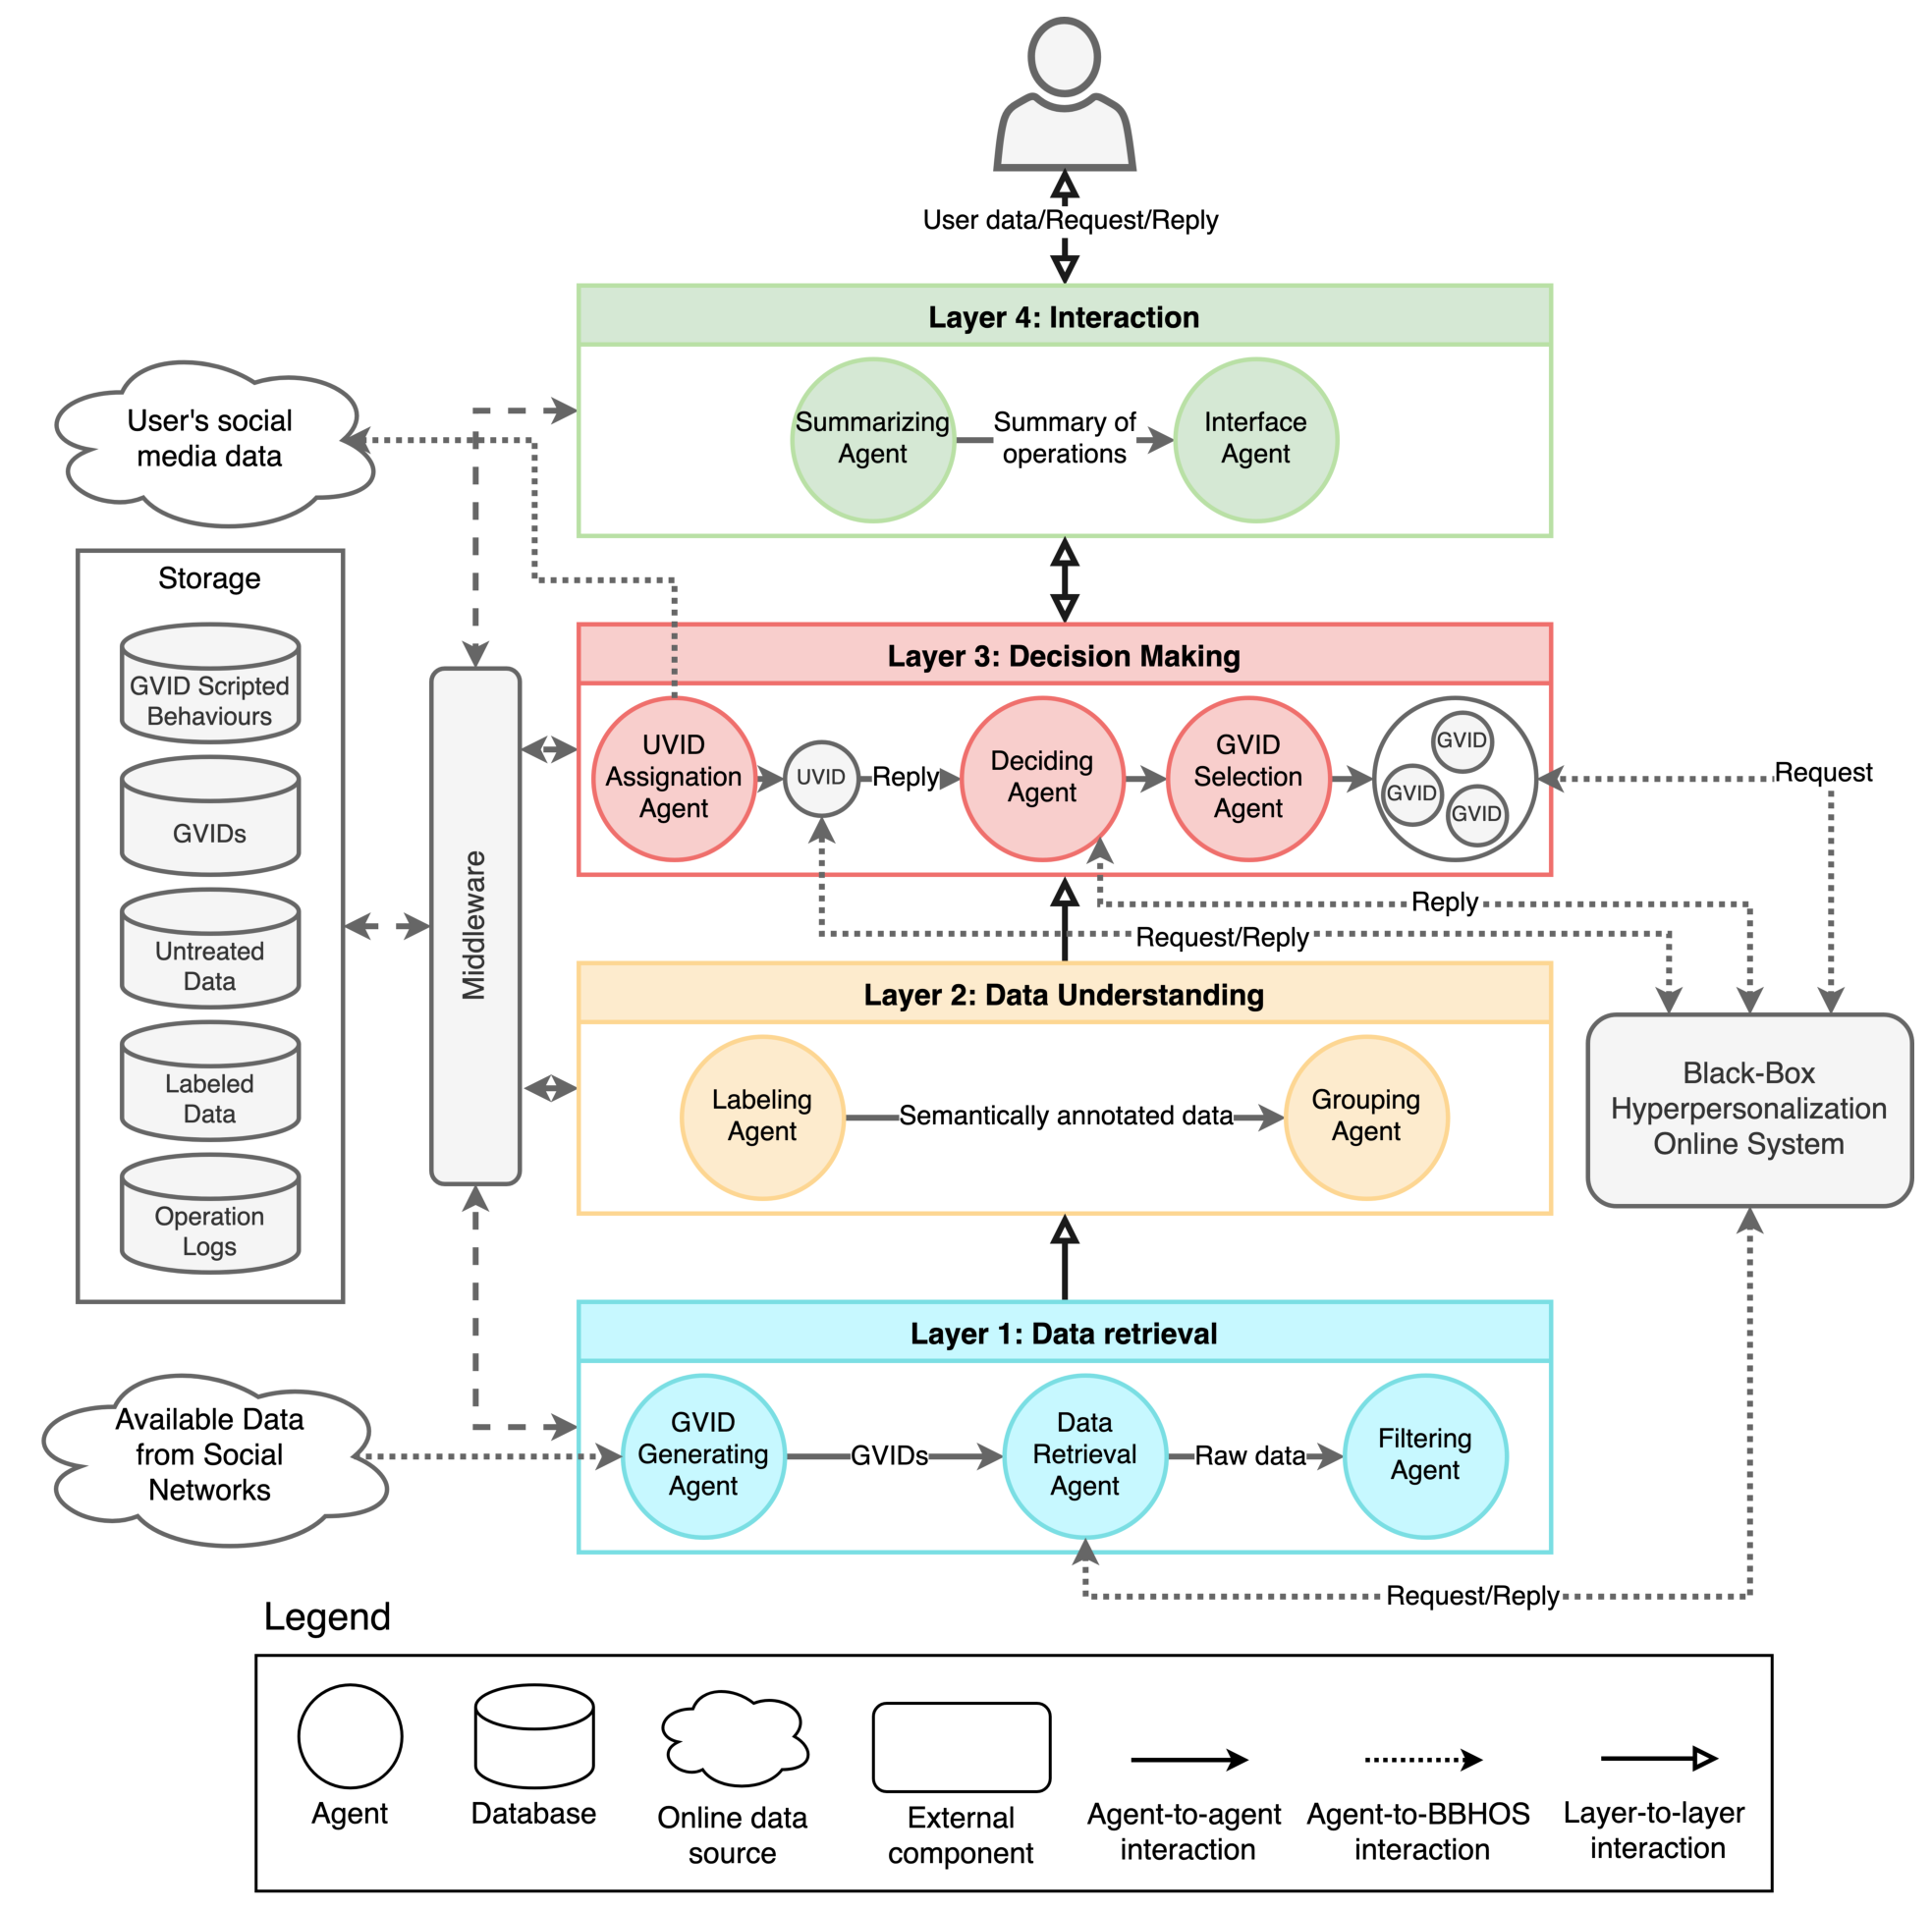
\includegraphics[width=.9\linewidth]{6_kbsextractiondl/figures/Overview_MAS.eps}
    \caption{Overview of the proposed hierarchical multi-agent system.}
    \label{fig:overview_mas}
\end{figure}

\subsubsection*{Layer 1: Data retrieval}
The first layer of the MAS comprises the operations related to the creation of GVIDs, as well as the BBHOS data extraction. This layer sets the purpose and goal of the system, selecting the BBHOS to study and the behaviour of the GVIDs. Three agents can be identified in this layer:
\begin{itemize}
    \item \textit{GVID generating agent.} Two elements are considered by this agent to generate the GVIDs, providing them with unique features and enabling the realistic emulation of the behaviour of real-life users. The first element are the core GVID features, which are stored in the system. These features include static treats such as gender, age, name, location, or interests. 
    
    Since static features are not enough to realistically emulate the behaviour of a user, social media data is also scrapped to generate user profiles. This data is collected \textit{ad-hoc} from external sources and its not stored in the system. Natural Language Processing (NLP) techniques are used to analyze and extract relevant information from this data, such as topic modeling \citep{Alghamdi2015} or sentiment analysis \citep{sentimentanalysis}. Information such as preferences, opinions, or interests can be extracted from this data, which can then be added alongside the static traits of the GVIDs to generate more complex, human-like behaviours. GVIDs are stored, and subsequently used by the superior layers of the system. 
    
    \item \textit{Data retrieval agent.} GVIDs interact with the BBHOS by making requests and receiving responses, which are aligned with their features and behaviors. This agent orchestrates and supervises the interactions between the GVIDs and the services, collecting the data generated in the process. Data can have different different formats, according to the targetted BBHOS, ranging from plain text to video files. Collected data is stored for further analysis, as it can be used to redefine the static traits of the GVIDs.
    
    As BBHOS are online systems and are subject to network-related issues, which need to be corrected before transmitting the data to the next agent. Hence, this agent also performs operations such as duplicate or corrupted data removal. 
    
    \item \textit{Filtering agent.} This agent receives the interaction data between the GVIDs and the BBHOS, and classifies it according to its format (e.g., image, text, or audio). Filtering and homogenization operations are performed to extract relevant content from the received data and to facilitate the usage of data understanding processes. According to the data format, suitable filtering operations may be required, such as normalization or text preprocessing. This agent only considers formal aspects of the content.
\end{itemize}

\subsubsection*{Layer 2: Data understanding}
Data understanding processes are needed to extract knowledge from the outputs of the interactions between the GVIDs and the BBHOS. The second layer of the MAS deals with the procedures required for this task. General knowledge on the behavior of the BBHOS can be inferred from the analysis of the content fed to each particular profile (encoded on the GVIDs). Two agents comprise this layer:
\begin{itemize}
    \item \textit{Labelling agent.} This agent annotates, classifies, and extracts knowledge from the collected interaction data. Due to the heterogeneity amongst data types, suitable approaches are required to effectively extract knowledge from the unstructured data. Multi-label classification using Convolutional Neural Networks (CNNs) \citep{He2015DeepRL,CNNRNN} can be used for image treatment, detecting the elements included in an image. CNNs can also be used for audio and video classification \citep{HersheyCEGJMPPS16}. For further processing, audio can be transcribed \citep{speechrecognition} to enable text operations. 
    
    The majority of the responses generated by the BBHOS are textual, thus requiring a more profound analysis than the aforementioned data formats. Multiple NLP techniques can be considered to analyze textual data from distinct perspectives. Text classification techniques \citep{MIRONCZUK201836} may be suitable to categorize the retrieved content. Topic modelling \citep{pmlr-v15-nallapati11a,Alghamdi2015} enable finer-grained classification and content analysis. Additionally, document clustering, as well as text summarizing techniques \citep{Neto00documentclustering,YOUSEFIAZAR201793,Oikonomakou2005} can be used to simplify and group the data, facilitating its comprehension.
    
    The annotated data is then stored in the system. As most of the state-of-the-art approaches for the aforementioned tasks rely on deep learning models, periodical retrainings may be needed to keep the models updated.
    
    \item \textit{Grouping agent.} While BBHOS are opaque, associative patterns may be inferred based on the responses provided to each particular GVID. Furthermore, GVIDs can be grouped based on the similarity of their targeted responses. This agent establishes GVID aggregation based on this information, using a hierarchical approach ranging from specific to general. Therefore, heterogeneity between the lower level clusters is maintained, while converging into a single aggregation in the final top level. GVID aggregations are stored in the system.
\end{itemize}

\subsubsection*{Layer 3: Decision Making}
In this layer, the user's data input is collected, processed, and sent to the final interaction layer. While the previous two layers follow a forward-only criterion, where the data flows from inferior to superior layers, this layer has a bidirectional flow. This layer can therefore be considered the core element of the system, and its execution is triggered directly by the user. This layer comprises three agents:
\begin{itemize}
    \item \textit{UVID assignation agent.} This agent creates and deploys a virtual identity that represents the real user within the system, referred to as the \textit{User Virtual Identity} (UVID). The UVID serves as an intermediary between the BBHOS and the user, protecting the user from potential privacy invasions. Similarly to GVIDs, the static information provided about the user is complimented with available social media data, whose recollection must be approved by the user. Moreover, the UVID also encodes the user's specifications on the content, thus serving as a filter. 
    
    \item \textit{Deciding agent.} Once the UVID is deployed, it interacts with the BBHOS. If the retrieved content meets the user's specifications, the response is then transferred to the superior layer, where the user can approve it. If not approved, this agent passes this information to the \textit{GVID selection agent}, which querys the BBHOS generating a new set of responses. This agent is aware of the user's requirements and decides which, if any, of the returned responses are suitable. If there are no valid responses, this agent reenacts the query to the BBHOS to receive new responses. This process is iteratively performed until the user indicates the validity of the response, or until no GVID aggregations remain.
    
    This agent orchestrates the interactions between the GVIDs and the BBHOS and collects the information from the real user and distributes it to the following agent. The data generated by this agent is also stored for further analysis.
    
    \item \textit{GVID Selection Agent.} If the response received by the UVID does not satisfy the user requirements, new responses are required as shown in Figure \ref{fig:overview_mas}. A new GVID set is selected if the \textit{deciding agent} sends a negative response. Since a specific-to-general approach is considered, similar GVID aggregations are first selected. If the user professes a strong rejection on the previous BBHOS response, then the agent may select a polar opposite GVID set in the following iteration.
    
    The initial GVID set is selected according to the similarity between the UVID and the existing GVID sets. As GVIDs are arranged hierarchically, a nearest neighbour criterion can be used. Thus, the aggregation containing the most similar GVID to the UVID is selected in the first place.

    \begin{figure}[t]
        \centering
        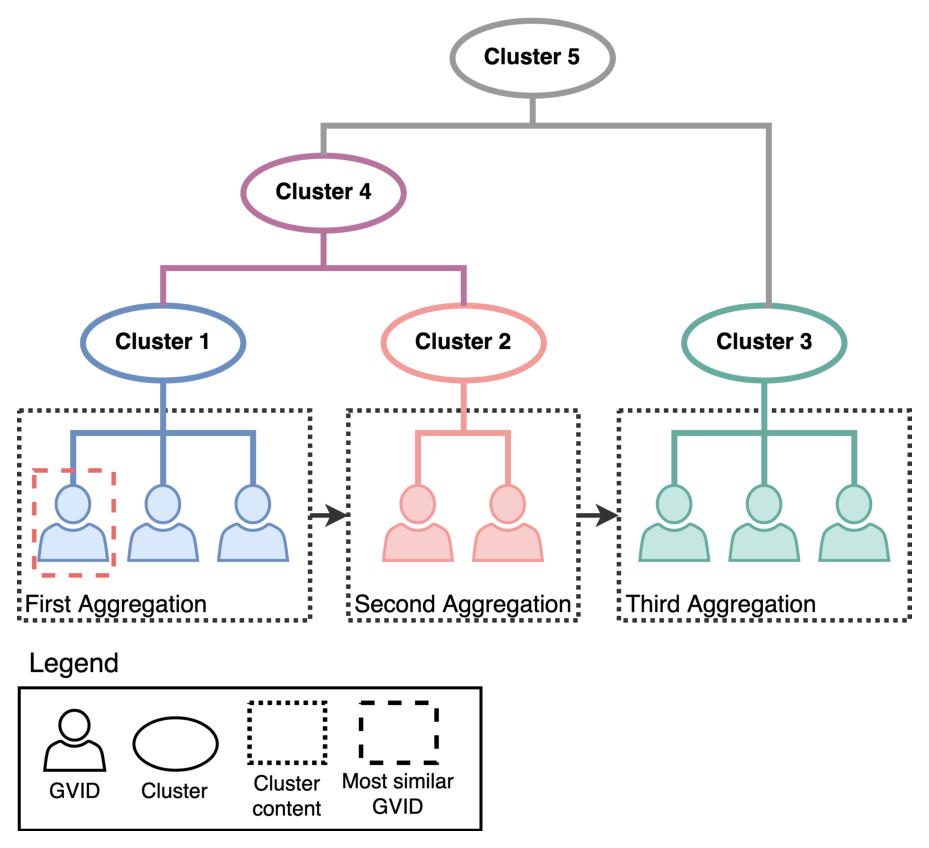
\includegraphics[width=.65\linewidth]{6_kbsextractiondl/figures/GVID_clusters.eps}
        \caption{Example of the GVID selection procedure.}
        \label{fig:gvid_selection}
    \end{figure}
    
    Figure \ref{fig:gvid_selection} depicts the general selection procedure. The GVID with the highest similarity to the UVID belongs to \textit{cluster 1}. Therefore, \textit{cluster 1} is selected as the initial GVID set. Then, the superior level of the hierarchy is explored (\textit{cluster 4}), which is composed of clusters 1 and 2. As \textit{cluster 1} has already been selected, \textit{cluster 2} would be selected as the next GVID aggregation. If the user does not express a strong disagreement with the provided responses, the system follows the specified hierarchical order to select the following aggregations.
\end{itemize}

\subsubsection*{Layer 4: Interaction}
Finally, an interaction layer is included to present the result of the operations performed in the inferior layers to the user. The data flow in this layer is also bidirectional, as the user not only receives, but introduces information in the system. User input is key to the system, as it conditions its behaviour. The agents of this layer determine what and how the content is displayed to the user. They also collect input from the user and forward it to the inferior layers.

\begin{itemize}
    \item \textit{summarizing agent.} To maintain the system's transparency, both the output and the log of the operations required for its generation are provided to the user. This agent extracts the logs of the iterations required by the \textit{deciding agent} to reach its final reply, and summarizes the most relevant information. Alongside the output, this agent generates a simple, user-readable record on which GVID received each response, as well as how many iterations were required. Thus, the real user can be conscious of whether the final response was obtained by the UVID or a different user profile (GVID).
    
    \item \textit{Interface agent.} User input is essential for the behavior of the system at its superior level. Appropriate mechanisms to interact with the user and correctly fulfill their requirements are needed. The communication with the user is established bidirectionally, implying that the system not only collects the user's input, but also generates an output that must be clear and readable. Therefore, this agent serves as a direct intermediary between the user and the system. The user's input is collected and transmitted to the lower layer for processing. Besides, this agent receives the output from the \textit{summarizing agent} containing the final BBHOS response and operation logs. This content is then displayed to the user in a simplified and visual format.
\end{itemize}

\subsubsection*{Storage units}
As depicted in Figure \ref{fig:overview_mas}, storage units serve as a sharing point for all MAS layers. The data generated during the system execution is heterogeneous, coming from different sources and in different formats. Five distinct databases are set to suit the different data types generated within the system:
\begin{itemize}
    \item \textit{GVID scripted behaviors.} Unique features are required to create a variety of user profiles to analyze the behaviour of BBHOS. These features refer to mid-term information, such as interests or age, which remains static throughout the execution.
    
    \item \textit{Untreated data.} This unit stores data extracted from the interactions between the GVIDs and the BBHOS in the first execution stages. The responses obtained from the BBHOS can then be used to redefine the behavior of the GVIDs.
    
    \item \textit{Labeled data.} Once untreated data has been filtered, categorized, and annotated is stored in this database. This data can then be used to periodically retrain the models in the \textit{labeling agent} to keep the system updated. 
    
    \item \textit{GVIDs.} GVIDs are at the core of the system and used by multiple agents of the system across different layers. Therefore, it is critical to ensure their persistence and accessibility. As well as the single GVIDs generated in the first layer of the system, the aggregations obtained after performing hierarchical clustering is also stored within this unit. If there is a change in the GVIDs, a reaction to the \textit{GVID generating agent} is unchained, initiating the execution of the autonomous level of the MAS.
    
    \item \textit{Operation logs.} A log of the communications between the GVIDs and the selected BBHOS is saved. The data generated from these interactions enables the extraction of associative patterns that enable understanding over the BBHOS. These logs are generated in the third layer and used in the fourth for summarization.
\end{itemize}

Additionally, there is a \textit{middleware} between the databases and the agents that orchestrates and supervises the introduction and extraction of data from the different databases. The middleware also ensures data persistence and avoids concurrency issues.

\subsection{Data Flow}\label{6_sec:subsec:data_flow}

\begin{figure}[t]
    \centering
    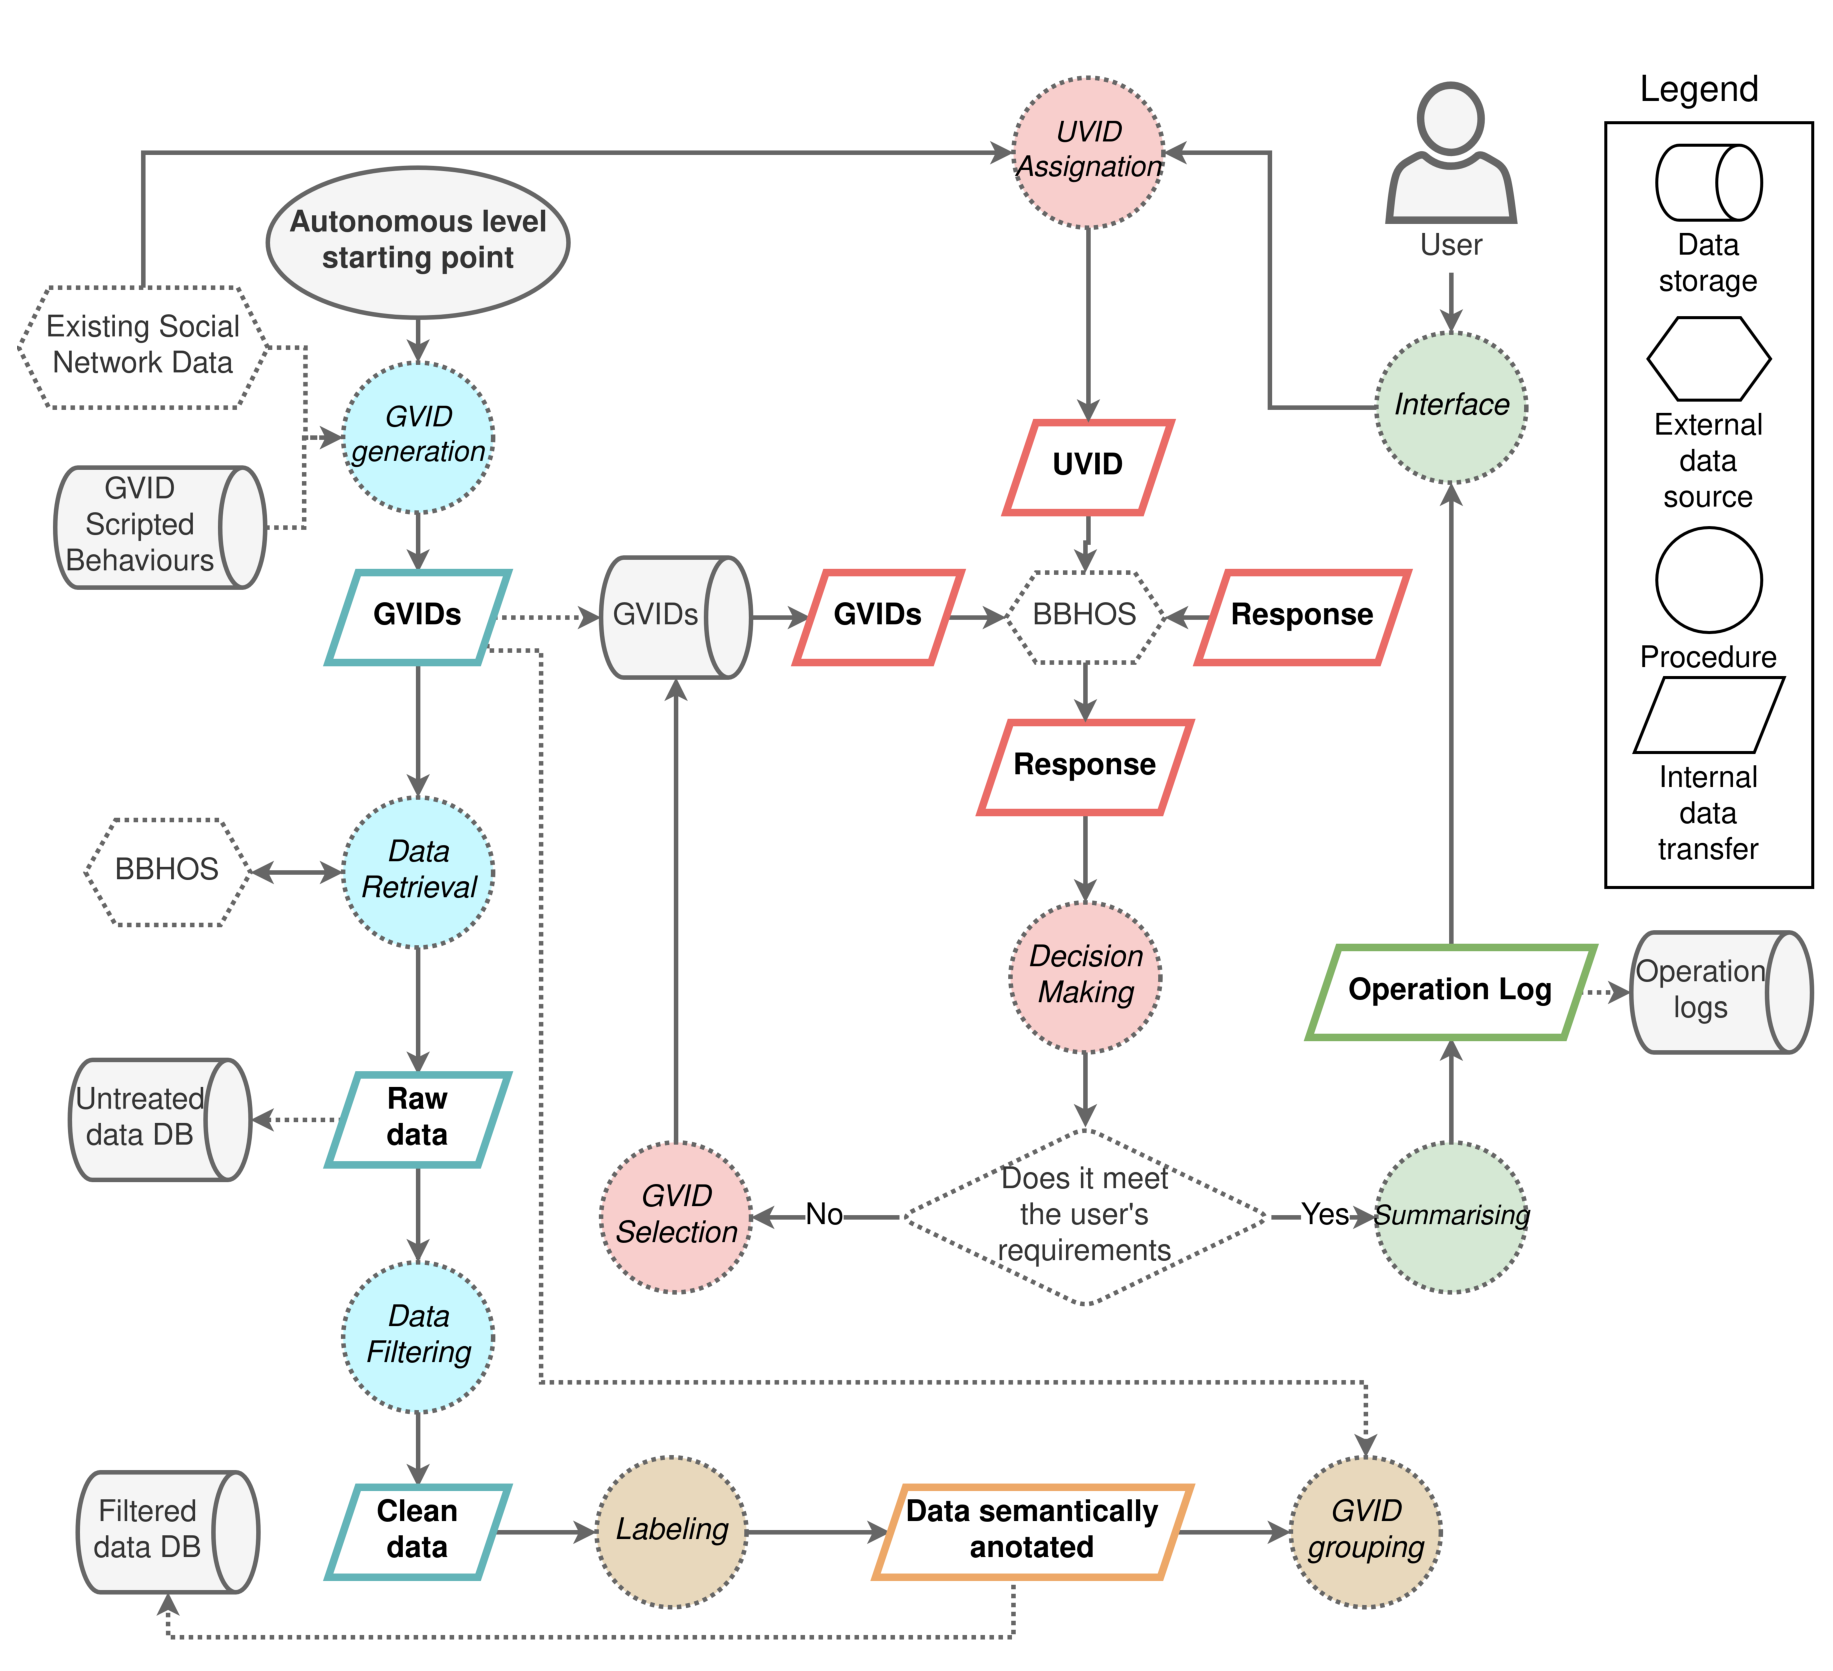
\includegraphics[width=\linewidth]{6_kbsextractiondl/figures/Data_flow.eps}
    \caption{Data flow of the proposed MAS. }
    \label{fig:data_flow_mas}
\end{figure}

Figure \ref{fig:data_flow_mas} depicts the data flow of the proposed MAS. Once the autonomous level of the system initiates, GVIDs are generated from a combination of scripted behaviours and existing social network data. The generated GVID set is then stored in the GVID database. GVIDs then interact with the BBHOS, receiving a set of responses in raw format, which are also stored for further analysis and GVID behaviour correction. 

Response data at this stage remains untreated, containing both relevant and irrelevant information. This data is first classified according to its format into video, audio, image, and text to facilitate its annotation and analysis. Appropriate filtering and homogenization operations are performed on the data, according to its format. Images are resized and normalized, while markup and stopword removal is performed on textual data. Filtering and cleaning the data not only eases the annotation, but also considerably reduces its size. The models in the \textit{labeling agent} then annotate the filtered data and store it in its corresponding database. Hierarchical clustering is then performed to aggregate the GVIDs with respect to the content of their responses. GVID clusters are also stored in the GVID database.

The previous operations belong to the autonomous level and are subsequently executed without any user interaction. In the second level of the system, comprised by layers three and four, the user is the entry point, and its interaction with the system triggers its execution. The user accesses the system from the interface, specifying a set of goals and specifications. Then, the UVID is generated. The UVID then interacts with the BBHOS, receiving a targeted response. If this response meets the user's requirements, it is then summarized and forwarded to the user using the \textit{interface agent}. On the contrary, if the user rejects the response or it is not aligned to the specified requirements, a set of GVIDs are selected, repeating the same request over the BBHOS. Once the user agrees with a response, the user-triggered level of the system is suspended until further interaction.

\subsection{Case Study}\label{6_sec:subsec:case_study}


This Section presents a case study to illustrate the proposed architecture. This case study aims to provide a clearer and deeper insight on the interactions and data transfer between agents, giving a complete overview on the behavior of the system. 

\begin{figure}[t!]
    \centering
    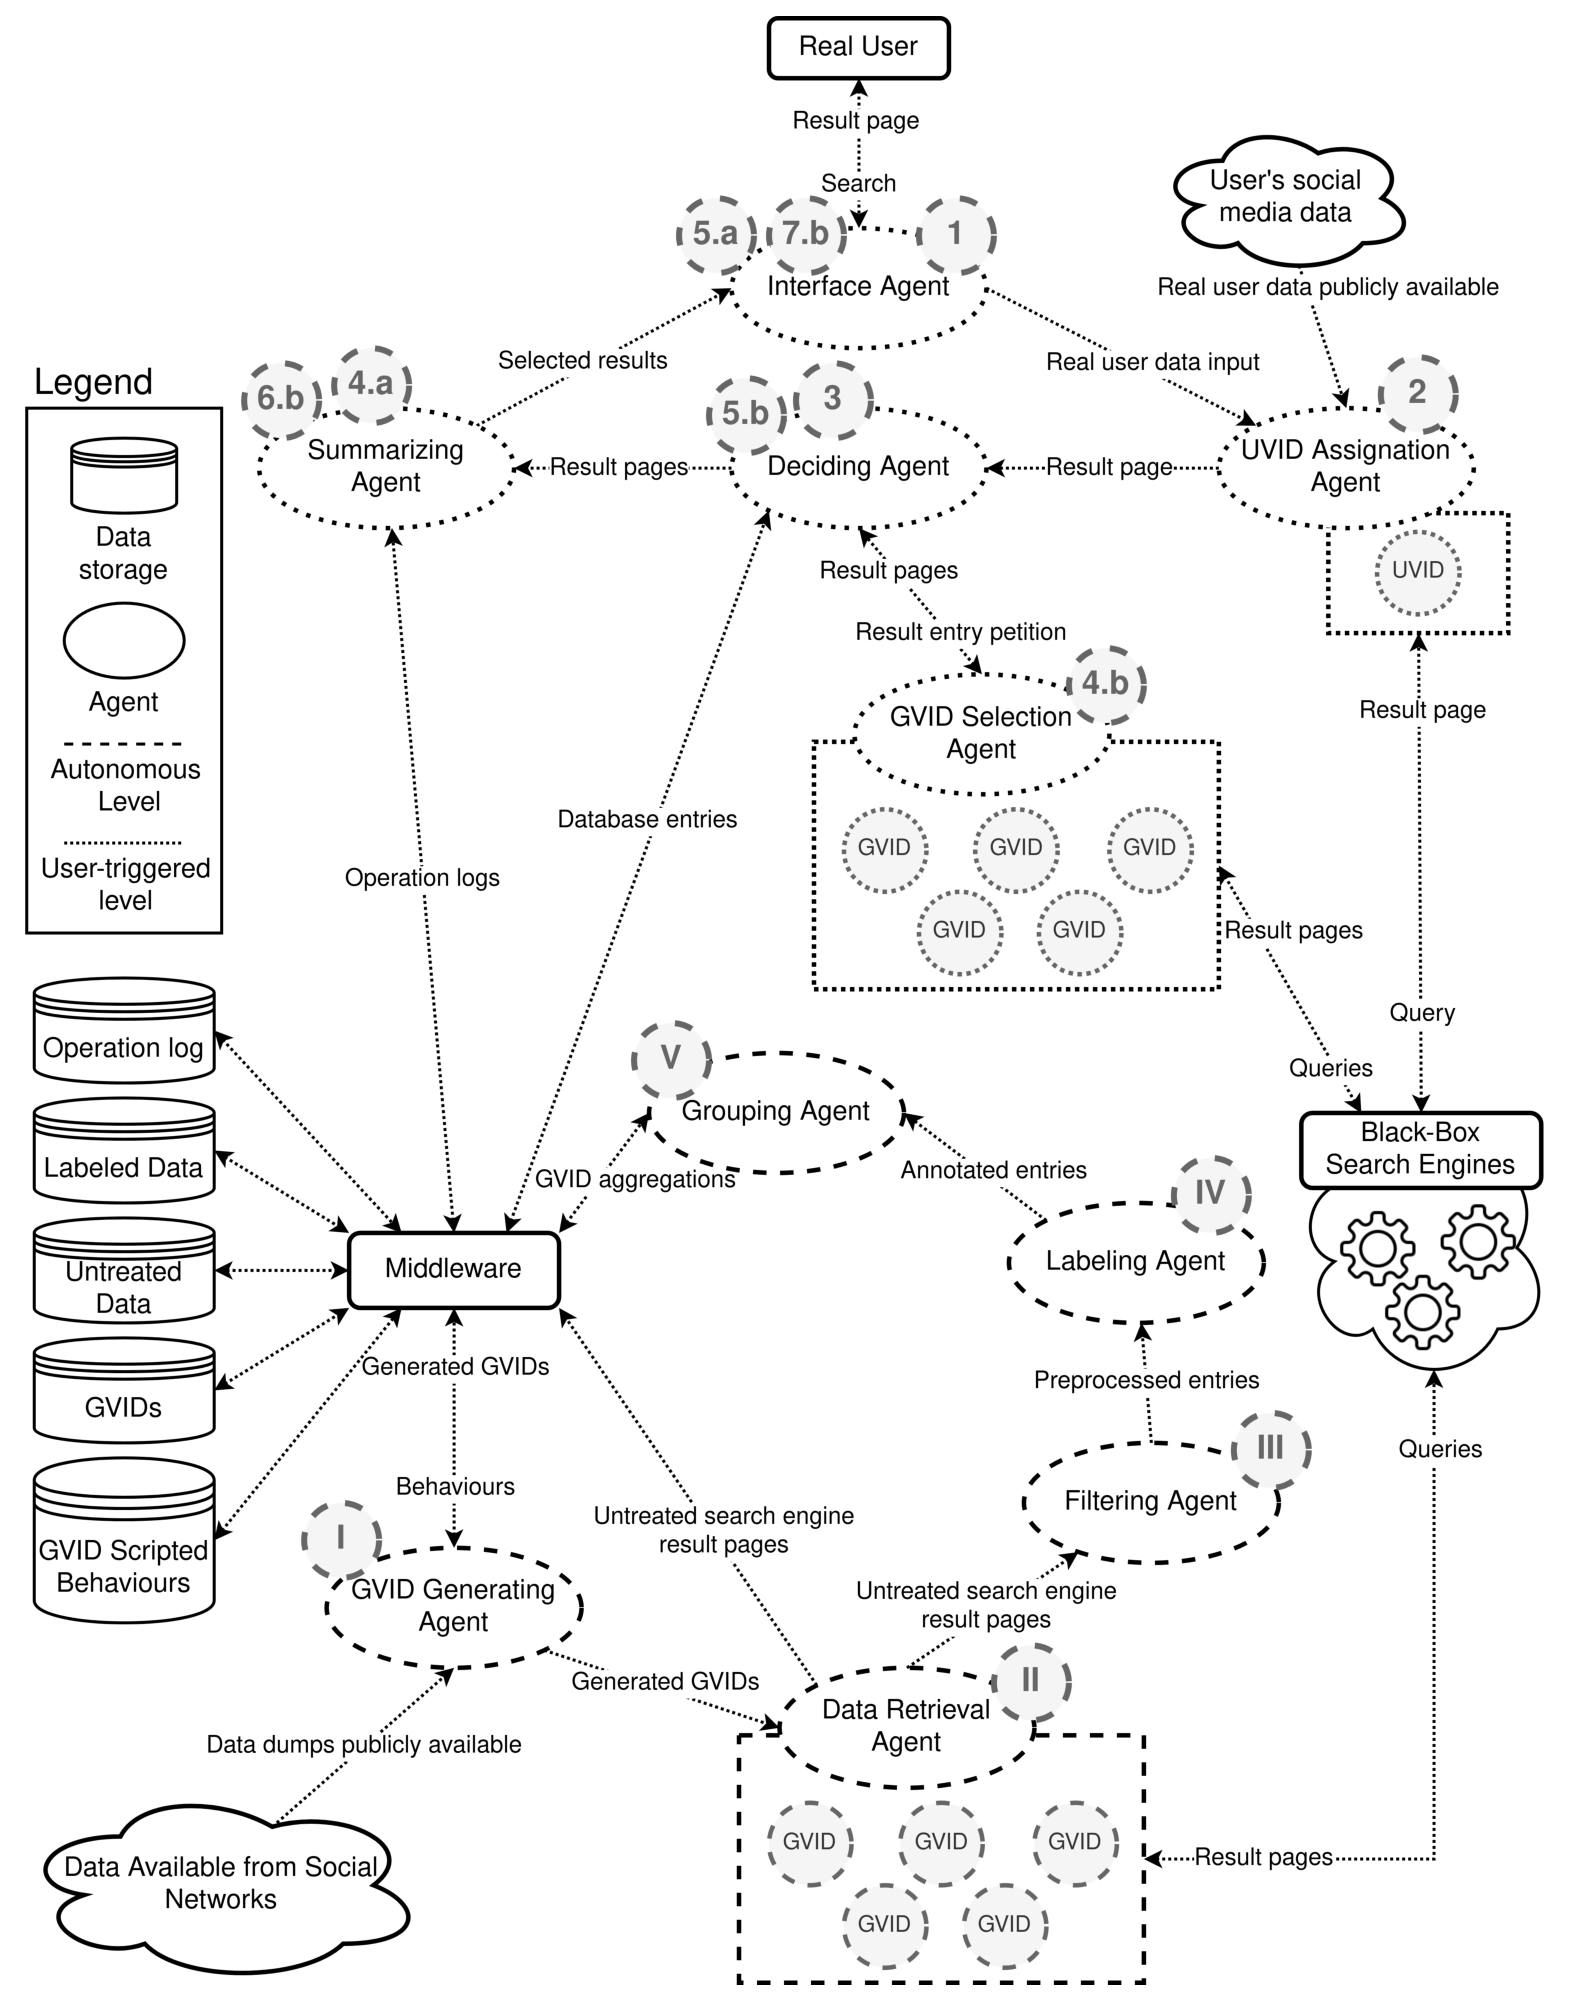
\includegraphics[width=.89\linewidth]{6_kbsextractiondl/figures/Use_Case.eps}
    \caption{Use case of the proposed architecture.}
    \label{fig:mas_use_case}
\end{figure}

The case study focuses on the analysis of the behaviour of search engines. Specifically, on the relevance of the entries on the first result page. From the perspective of the user, the results that best fit the search query should be featured on the initial result page, independently from the employed search engine. However, this statement is not consistently met across search engines as the result may vary not only between search engines, but also between users. Moreover, most search engines feature advertising content amongst the top results, even when this content is unrelated to the search query. Therefore, this content should be detected and replaced by relevant result entries.

The considered case scenario meets the following specifications:
\begin{itemize}
    \item The goal of the system is to detect, analyze, and optimize result entries in search engines.
    \item Multiple search engines are selected, acting as the BBHOS.
    \item A reduced set of GVIDs is selected. Each GVID has distinct features to maximize heterogeneity in the BBHOS results.
    \item The system determines which results are related to the user's query, removing those entries that contain unrelated content, such as adverts.
\end{itemize}

As the architecture is divided into two distinct levels, the interactions between the agents on each level are presented separately. Figure \ref{fig:mas_use_case} illustrates the present use case. Operations related to the autonomous layer are numbered using Roman numerals, while Arabic numerals denote the operations user-triggered layer. Two distinct scenarios can occur based on the outcome of the \textit{deciding agent}, identified with letters \textit{a} and \textit{b} to designate the execution order of the agents.

\subsubsection*{Autonomous level}
In this level, the system gathers data from different search engines to be processed by the agents. The workflow is as follows:

\begin{enumerate}[label=\Roman*.]
    \item The \textit{GVID generating agent} collects tha available social network user data dumps and extracts a set of \textit{N} GVID behaviors from the database. The collected social network data is then shuffled and distributed into \textit{N} different sets, each containing information such as tweets, reviews or opinions. Sentiment analysis and topic modeling are then performed over the sets to extract interest and opinions. This information is then combined with the GVID scripted behaviors to generate the final GVID set. The generated GVIDs are then stored in the database.
    
    \item Once the GVIDs are created, the \textit{data retrieval agent} selects a set of search engines to act as BBHOS, as well as defining the browsing terms to be queried. The browsing term set is composed by the topics extracted in the prior step. Each GVID does the same number of searches, and multiple GVIDs query the same term across the different engines. This enables the analysis of the results returned when the same term is browsed on different search engines and those obtained by different GVIDs when the search terms and engine are the same. The obtained responses are stored in the corresponding database.
    
    \item The result pages received by the GVIDs are then forwarded to the \textit{filtering agent}, which performs the data preprocessing. The collected data is in HTML format, thus containing several moot elements, such as markup text, references or symbols. The following operations are performed to clean the raw result pages: entry extraction, HTML and JavaScript markup removal, empty word removal and non-alphanumeric character removal. A set of clean result entries is obtained as outcome.
    
    \item As previously stated, search engines tend to merge advertising and valid result entries within the same page. Invalid entries should be detected and discarded, such that the user is only presented with entries that correspond to valid search results. The \textit{labeling agent} receives the result entry set from the previous agent and classifies entries into real result and advertisements. This problem can be subsequently treated as binary text classification. Labeled result entries are stored in the labeled data storage.
    
    \item Finally, GVIDs are hierarchically aggregated by their result entries to further analyzed the behaviour of the search engines. The \textit{grouping agent} receives labeled entries and aggregates them following a hierarchical approach. As a result, GVIDs are grouped based on the result entries provided for each of them by the different engines. Information about the behavior of the search engines can then be extracted, such as which profiles are the most prone to receive advertising content, which engine includes the least amount of irrelevant content amongst its entries, or whether the results provided by the same engine on the same search vary across GVIDs. GVID aggregations are also saved in the GVID database.
\end{enumerate}

\subsubsection*{User-triggered level}
Once the autonomous level finishes its execution, the system remains suspended until a user makes a request. In this example, the request is a search query that the user inputs into a search engine. When the user makes the request, the user-triggered level of the system initiates its execution:
\begin{enumerate}
    \item The \textit{interface agent} collects the user's query, alongside with the needed user information. This input is sent to the \textit{UVID assignation agent} for further processing.
    
    \item The user's virtual identity, or UVID, is generated from the contextual information of the user, alongside with the publicly available social media information. The same procedure followed to generate the GVIDs is employed to generate the UVID. The UVID makes the user's search request, hindering the search engine from extracting contextual information about the user that could result in a privacy breach or lead to unfitting responses.
    
    \item The UVID executes the user's search query on the search engine. Then, the \textit{deciding agent} receives the result pages, determining whether the entries returned by the engine fit the user's request. Result entries are extracted from the result page to analyze their validity. These entries are filtered following the same procedure from step III. Then, the text classification model is used to discern advertisements from real result entries. At this point, two different scenarios can occur based on whether the result entries are real results (\textit{Scenario A}) or not (\textit{Scenario B}). 
    
    \paragraph{Scenario A}
    \begin{enumerate}
        \item [4.a] If the results provided by the engine to the UVID are relevant, meaning that no advertisements have been detected within the entries, the \textit{summarizing agent} compiles them for the user (e.g., removes duplicate entries).
        
        \item [5.a] Finally, the \textit{interface agent} builds a result page from the final result entry set and displays it to the real user. The constructed result page is formatted employing an adequate layout to present the information to the user in a clear and comprehensible way.
    \end{enumerate}
    
    \paragraph{Scenario B}
    \begin{enumerate}
        \item [4.b] If there is unrelated content amongst the results, the \textit{deciding agent} discards those entries and makes a petition to the \textit{GVID selection agent} to obtain new, valid entries to replace the removed ones. A set of GVIDs is selected following the hierarchical selection criteria, repeating the same query on the search engine. The new responses are sent back to the \textit{deciding agent}.
        
        \item[5.b] The new set of entries obtained by the GVIDs is analyzed by the \textit{deciding agent}, following the procedure presented in the step 3. The results that better fit the search query are then selected to replace the discarded entries. If no relevant results are found, the agent makes a new petition to the \textit{GVID selection agent}, repeating the process until valid result entries are obtained.
        
        \item [6.b] The generated result entry set, composed by the entries received by the UVID and the GVIDs, is transferred to the \textit{summarizing agent}. Aside from summarizing the result entries, this agent also generates a log comprising the operations required to obtain the final result entry set, identifying the GVID that originated each result.
        
        \item [7.b] The \textit{interface agent} composes a result page from the final entry set and displays it to the user, finishing the execution of the user-triggered layer of system.
    \end{enumerate}
\end{enumerate}

\subsection{Design Compliance}\label{6_sec:subsec:design_compliance}

%\section{A Hierarchical Multi-Agent Architecture Based on Virtual Identities}

%\section{Design Compliance I}



%%-----
%\section{Explainability on Knowledge Graph Completion}

%\section{GEnI: A Model-Agnostic Framework for Generating Explanations and Insights on Link Predictions}

%\section{Design Compliance II}
\section{Summary}